\documentclass[12pt,a4paper,twoside]{article}
\usepackage{labor}
\begin{document}

%fill for cover and header creation
\newcommand\laboratorynumber{2}
\title{3D Kino/Polarisation}
\newcommand\supervisor{Ditlbacher, Harald}
\newcommand\groupnumber{42}

\newcommand\participantonelastname{Eisner}
\newcommand\participantonefirstname{Nico}
\newcommand\participantoneid{12214121}
\newcommand\participanttwolastname{Waldl}
\newcommand\participanttwofirstname{Philip}
\newcommand\participanttwoid{12214120}
\author{\participantonelastname \ \& \participanttwolastname}

\newcommand\degreeid{UB 033 678}
\newcommand\semester{23WS}
\date{21.10.2023}

%select correct course title
%\newcommand\coursetitle{Einführung in die \\ physikalischen Messmethoden}
%\newcommand\coursetitle{Laborübungen 1: \\ Mechanik und Wärme}
\newcommand\coursetitle{Laborübungen 2: \\ Elektrizität, Magnetismus, Optik}
%\newcommand\coursetitle{Fortgeschrittenen Praktikum 1: \\ Technische Physik}
%\newcommand\coursetitle{Fortgeschrittenen Praktikum 2: \\ Allgemeine Physik}

%\begin{titlepage}
   \begin{center}
       \begin{figure}[H]
            \begin{minipage}[h]{30mm}
                \centerline{
\includegraphics[height=15mm]{cover_nudes/tugraz.png}}
            \end{minipage}
            \hfill
            \begin{minipage}[h]{30mm}
                \centerline{
\includegraphics[height=15mm]{cover_nudes/nawi_graz.png}}
            \end{minipage}
            \hfill
            \begin{minipage}[h]{30mm}
                \centerline{
\includegraphics[height=15mm]{cover_nudes/uni-graz.png}}
            \end{minipage}
        \end{figure}
        
        \large{\emph{Institut für Experimentalphysik der Technischen Universität Graz \\
        \& Institut für Physik der Universität Graz}} \\
        \vspace{5mm}
        
        {\Huge \textbf{\coursetitle}}
        \vspace{5mm}
        
        {\huge \laboratorynumber: \thetitle}
    \end{center}
    
    \vfill
    
    \begin{table}[H]
        \LARGE
        \centering
        \begin{tabular}{r l}
            Betreuer:       & \supervisor \\
            Gruppennummer:  & \groupnumber \\
            \\
            Name:           & \participantonelastname, \participantonefirstname \\
            Matrikelnummer: & \participantoneid \\
            Name:           & \participanttwolastname, \participanttwofirstname \\
            Matrikelnummer: & \participanttwoid \\
            \\
            Kennzahl:       & \degreeid \\
            Datum:          & \semester \ | \thedate
        \end{tabular}
    \end{table}
    \vspace{4cm}
\end{titlepage}
\clearpage
\setcounter{page}{1}

%\maketitle %short title alternative

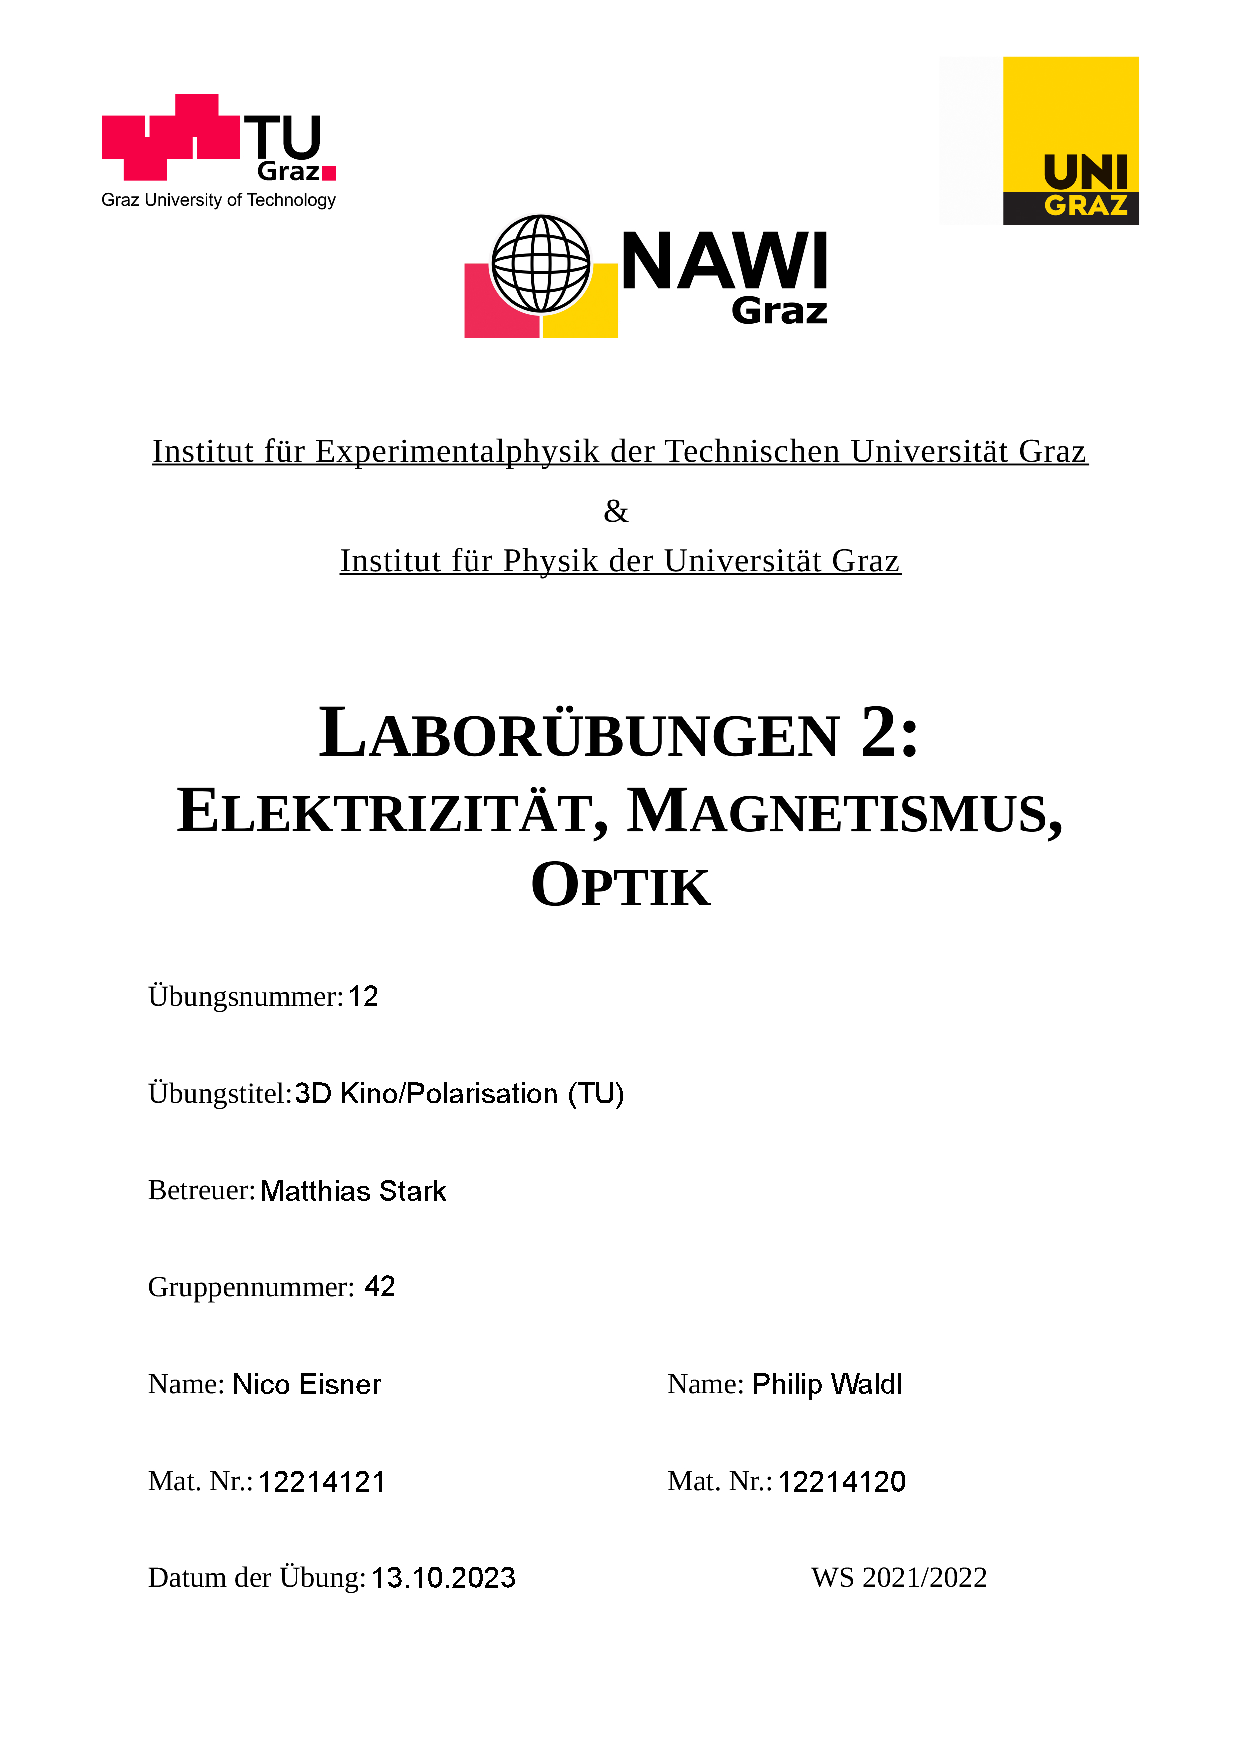
\includepdf[pages={1}]{../Deckblätter/Deckblatt_3DKino.pdf}

\tableofcontents
\newpage

\section{Aufgabenstellung} %jo beschreibn wos gmocht host ------------------------------
Das Experiment 3D Kino/Polarisation besteht aus folgenden Aufgaben. 
Im ersten Teil gilt es das Gesetz von Malus zu beweisen. 
Die Aufgabe im zweiten Teil ist es, die konzentration einer Zuckerlösung zu bestimmen. 
Anschließend wird mithilfe eines Handybildschirmes Spannungsdoppelbrechungen beobachtet. 
\\
Im Teil 3D Kino wird zuerst die Orientierung der Polarisator Folien einer 3D Brille bestimmt. 
Anschließend wird eine 3D Projektion mit dem RealD-verfahren erzeugt. 
\\
\\
Alle Informationen und Methodiken wurden uns von der Technischen Universität bereitgestellt \cite{teachcenter2}. 


\section{Voraussetzungen \& Grundlagen} %Grundlagen erklären, Formeln mit erklärung
Um das Gesetz von Malus zu beweisen, gilt es erst einmal dieses zu kennen. 


    \begin{equation}
        \label{eq:Gesetz von Malus}
        \centerline{$I = I_0 cos^2(\theta) = \vert E_0 \vert ^2 cos^2(\theta)$}
    \end{equation}

\noindent
Eine linear polarisierte Lichtwelle trifft auf einen Polarisator. Dabei ändert sich je nach Winkel $\theta$, unter dem das Licht auf den Polarisator fällt, die Intensität $I$. 
Dabei ist $I_0$ die Intensität des Lichtes vor Durchtritt des Polarisators. 
\\
Der Vektor wird in seine Komponenten zerlegt und parallel und senkrecht in Durchlassrichtung des Polarisators verschoben. 

\begin{figure}[H]
    \centering
    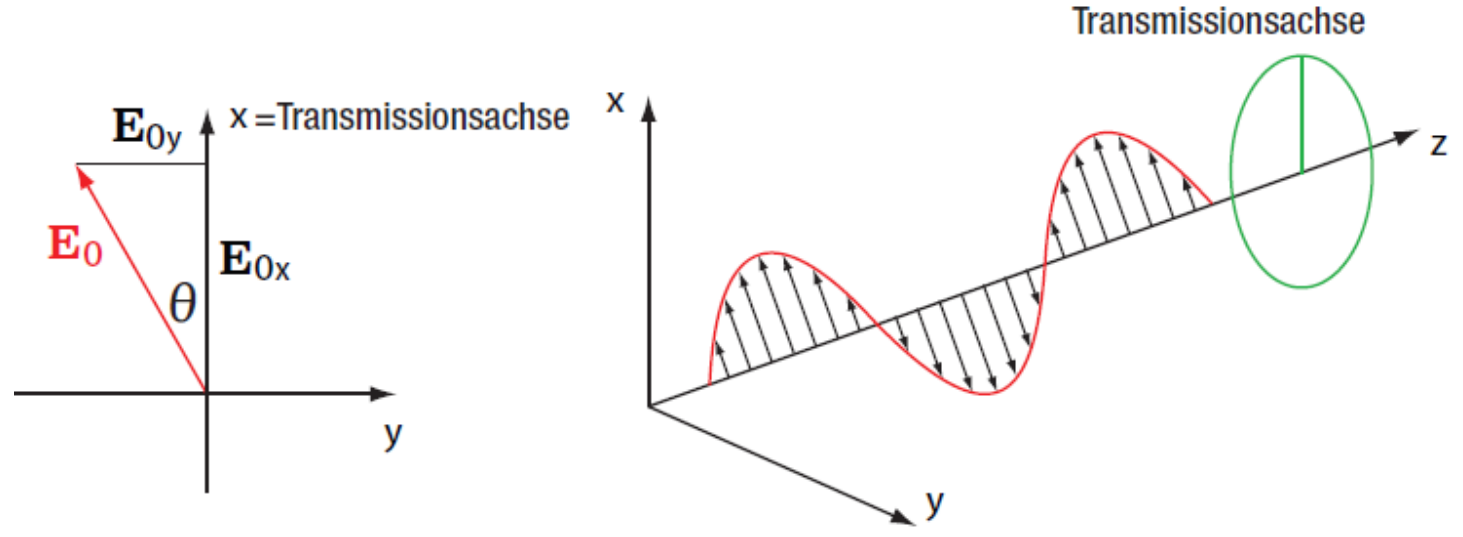
\includegraphics[width=0.6\linewidth]{nudes/Mallus.png}
    \caption{Aufteilung des Vektors einer linear polarisierten Lichtwelle durch den Polarisator. \\ Entnommmen aus Seite 3 Skriptum Polarisation \cite{teachcenter2}}
    \label{fig:Mallus Vektor}
\end{figure}

\noindent
Um die Konzentration der Zuckerlösung zu berechnen benötigt man die Länge des Zuckergefäßes, sowie den Winkel $\varphi$. Die Konzentration $c$ entspricht der stärke der Zuckerlösung. 

\begin{equation}
    \label{eq:Konzentration Zucker}
    \centerline{$\varphi = \varphi_0 cL$}
\end{equation}

\noindent
Die Zuckerlösung dreht die Polarisationsrichtung des Lichtes, da die Zuckermoleküle einen Drehsinn zeigen. 
Daraus folgt, zirkular polarisiertes Licht wird anders transmittiert. 
\\
\\
Durch Druck auf isotropische Materialien lässt sich ein Effekt hervorrufen, bei dem Licht je nach Ausbreitungsrichtung unterschiedlich transmittiert wird. Daraus folgen unterschiedliche Brechungsindizes. 
Übt man Druck auf ein Plastikteil aus, so erkennt man eine unterschiedliche Verspannung im Material, bzw einen unterschiedlichen Brechungsindex. 
Durch einen Polarisator kann dieser Effekt sichtbar gemacht werden. 
\\
\\
Einen 3D Effekt erzeugt man, indem man aus zwei verschiedenen Perspektiven aufgenommene Bilder überlagert und in die Augen des Betrachters leitet. 
Dabei ist jedoch wichtig, dass jeweils nur ein Bild in ein Auge fallen darf, um einen Tiefeneindruck zu erschaffen. 
Das gängigste Verfahren ist das RealD-Verfahren. Hierbei werden vor dem Projektor ein linearer Polarisator und ein $\lambda/4$ (Lambda viertel) Plättchen gestellt. 
Mit den richtigen Einstellungen erhält man für die Lichtwege rechtszirkulierte und für den anderen Weg linkszirkulierte Polarisation. \\
Die 3D-Brille reversiert den Prozess. Dort polarisert ein $\lambda/4$ Plättchen das Licht und trifft dann erneut auf einen Polarisator. 

\begin{figure}[H]
    \centering
    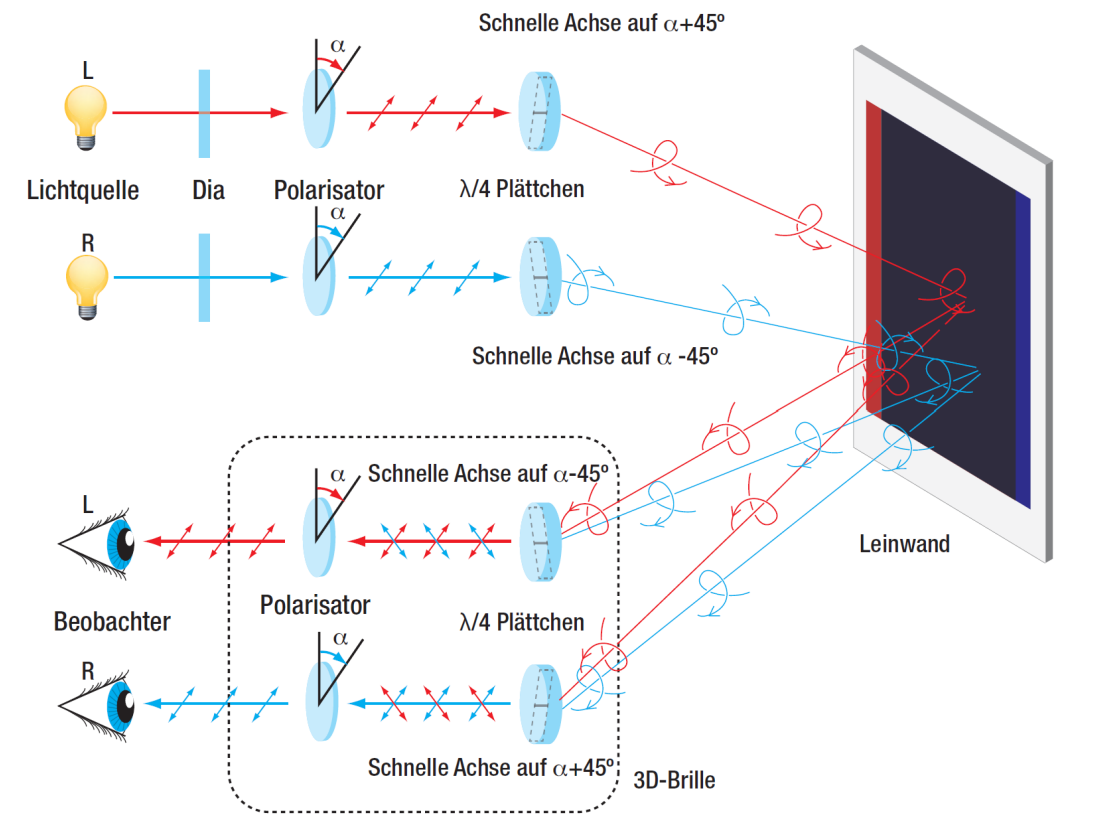
\includegraphics[width=0.6\linewidth]{nudes/3D.png}
    \caption{Darstellung einer 3D Projektion \\ Entnommmen aus Seite 5 Skriptum Polarisation \cite{teachcenter2}}
    \label{fig:3D Projektion schema}
\end{figure}

\section{Versuchsanordnung} %mit skizze kurz beschreiben ------------------------------

    \begin{figure}[H]
        \centering
        %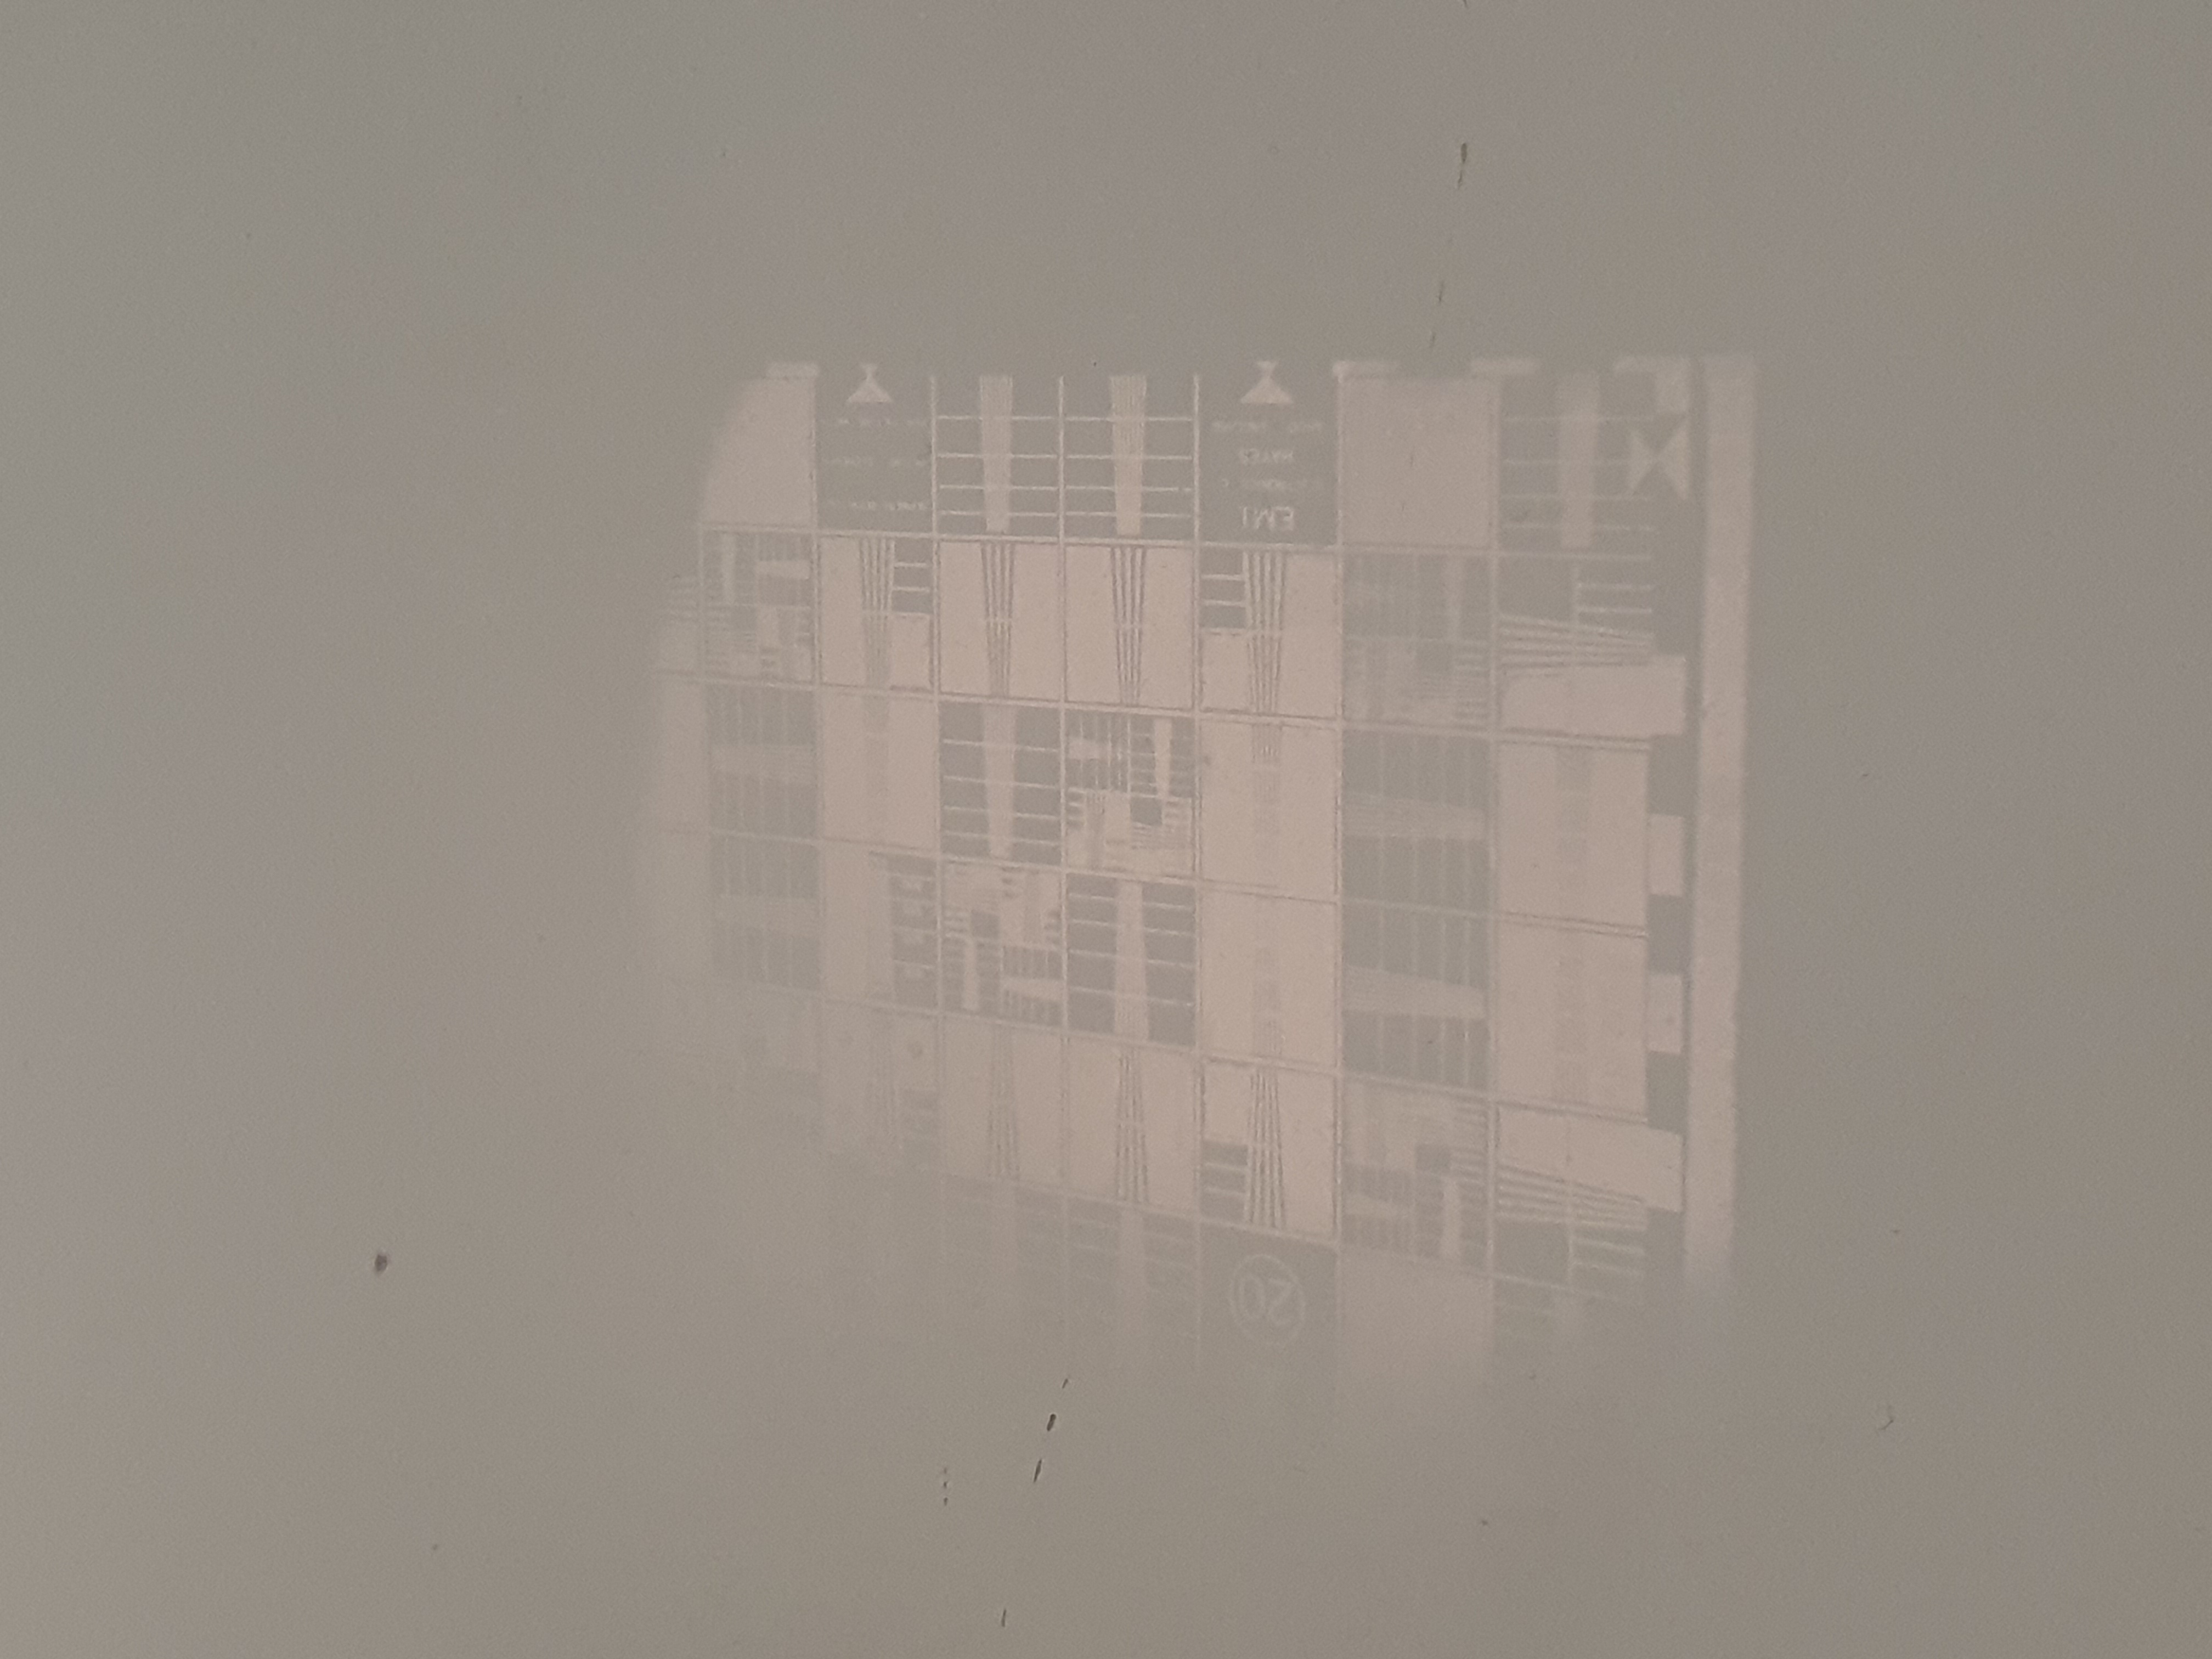
\includegraphics[width=0.6\linewidth, angle=-90]{nudes/bild.jpg}
        \caption{müll}
        \label{fig:müllbild}
    \end{figure}

\section{Geräteliste} %jo holt a listn ------------------------------

    \begin{table}[H]
        \centering
        \caption{Im Versuch verwendete Geräte und Utensilien.}
        \label{tab:geraete}
        \begin{tabular}{| l | l | l | l |}
            \hline
            Gerät   & Typ   & Gerätenummer  & Unsicherheit \\
            \hline
        \end{tabular}
    \end{table}


\section{Versuchsdurchführung \& Messergebnisse} %nachvollziehbar und klar dargestellt ------------------------------


\section{Auswertung und Unsicherheitsanalyse} %Nicht nur zahlen angeben ------------------------------

In der Auswertung werden zur erhöhten Genauigkeit durchgehend ungerundete Werte bis zu den Endergebnissen verwendet und nur zur Darstellung gerundet. \\
Zur Berechnung der Unsicherheiten wird, wenn nicht anders angegeben, die Größtunsicherheitsmethode verwendet.


\section{Diskussion} %diskussion der Unsicherheiten und Ergebnisse und evtl. verlgeich mit Literatur ------------------------------


\section{Zusammenfassung} %klare, übersichtliche vollständige beantwortung der Aufgabenstellung ------------------------------


\printbibliography[heading=bibintoc]
\end{document}
